\documentclass[10pt,a4paper]{article}
\usepackage[utf8]{inputenc}
\usepackage{amsmath}
\usepackage{amsfonts}
\usepackage{amssymb}
\usepackage{graphicx}
\usepackage[hidelinks]{hyperref} 
\usepackage{color}
\usepackage{xcolor}
\usepackage{caption}
\usepackage{subcaption}
\author{María Isabel Ruiz Martínez}
\title{Análisis ANOVA y primeras conclusiones}

%Ruta absoluta en formato tipo Unix (Linux, OsX)
\graphicspath{ {/home/maribel/Escritorio/5º DGIIM/TFG/Analysis-of-processes/documentation/images} }

\begin{document}

\maketitle

\listoftables
\listoffigures

\section{Descripción del dataset}

Los datos que se van a usar han sido recopilados por Luis Castillo Vidal y corresponden a la actividad de sus alumnos en la asignatura \href{https://www.ugr.es/estudiantes/grados/grado-ingenieria-informatica/desarrollo-basado-agentes-ing-software}{\color{blue}{Desarrollo Basado en Agentes}}.

El dataset, tras haber sido filtrados los registros erróneos, consta de 47828 filas correspondientes a los diferentes acciones de unos drones en una serie de mundos virtuales. En cada registro se detallan los siguientes atributos:
\begin{itemize}
\item \emph{year}: identifica el curso académico en el que se realizó dicha acción.
\item \emph{group}: grupo de prácticas que ha prograda al dron que acomete la acción.
\item \emph{date}: fecha en la que se lleva a cabo la acción.
\item \emph{map}: mundo virtual en el que se ha realizado la acción.
\item \emph{action}: indica el tipo de acción realizada.
\end{itemize}
% Dimesiones: 47828 registros, 5 columnas por registro.

En la Tabla \ref{table:1} se presentan los primeros seis registros del dataset. Además, en la Tabla \ref{table:2} puede apreciarse un resumen de los datos que tenemos.

% Muestra del dataset
% latex table generated in R 4.2.2 by xtable 1.8-4 package
% Wed Feb  1 15:07:17 2023
\begin{table}[ht]
\centering
\begin{tabular}{rlllll}
  \hline
 & year & group & date & map & action \\ 
  \hline
1 & 1516 & Achernar & 17/10/2015 19:41:45 & 0 & 0 \\ 
  2 & 1516 & Bellatrix & 17/10/2015 19:41:45 & 0 & 0 \\ 
  3 & 1516 & Cerastes & 17/10/2015 19:41:45 & 0 & 0 \\ 
  4 & 1516 & Denebola & 17/10/2015 19:41:45 & 0 & 0 \\ 
  5 & 1516 & Elnath & 17/10/2015 19:41:45 & 0 & 0 \\ 
  6 & 1516 & Furud & 17/10/2015 19:41:45 & 0 & 0 \\ 
   \hline
\end{tabular}
\caption{Muestra del dataset}
\label{table:1}
\end{table}

% Resumen del dataset que tenemos:
% latex table generated in R 4.2.2 by xtable 1.8-4 package
% Wed Feb  1 15:08:53 2023
\begin{table}[ht]
\centering
\begin{tabular}{lllll}
  \hline
     year &    group &     date &      map &     action \\ 
  \hline
Min.   :1516   & Length:47828       & Length:47828       & Min.   :0.000   & Min.   :0.000   \\ 
  1st Qu.:1516   & Class :character   & Class :character   & 1st Qu.:1.000   & 1st Qu.:1.000   \\ 
  Median :1617   & Mode  :character   & Mode  :character   & Median :3.000   & Median :2.000   \\ 
  Mean   :1700   &  &  & Mean   :3.834   & Mean   :2.325   \\ 
  3rd Qu.:1920   &  &  & 3rd Qu.:6.000   & 3rd Qu.:3.000   \\ 
  Max.   :1920   &  &  & Max.   :9.000   & Max.   :5.000   \\ 
   \hline
\end{tabular}
\caption{Resumen del dataset que tenemos}
\label{table:2}
\end{table}

La Figuras \ref{fig:boxplotmap} y \ref{fig:boxplotaction} muestran, respectivamente, los gráficos de caja y bigotes de las variables \emph{map} y \emph{action}.

\begin{figure}[!tbp]
  \begin{subfigure}[b]{0.49\textwidth}
    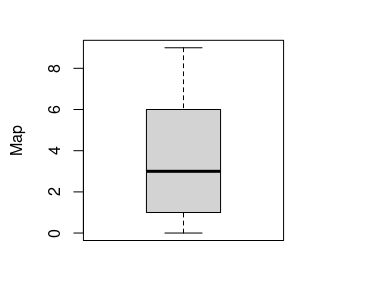
\includegraphics[width=\textwidth, height=\textwidth]{Rplot02.png}
    \caption{Gráfico de caja y bigotes de la variable \emph{map}}
    \label{fig:boxplotmap}
  \end{subfigure}
  \hfill
  \begin{subfigure}[b]{0.49\textwidth}
    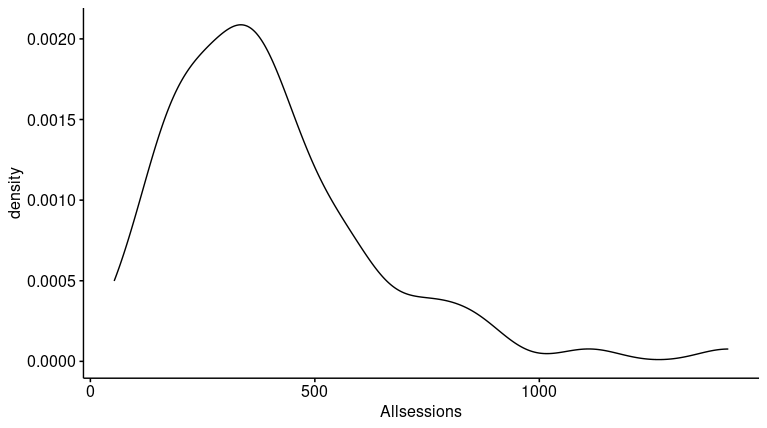
\includegraphics[width=\textwidth, height=\textwidth]{Rplot04.png}
    \caption{Gráfico de caja y bigotes de la variable \emph{action}}
    \label{fig:boxplotaction}
  \end{subfigure}
  \caption{Diagramas de caja y bigotes de las variables \emph{map} y \emph{action}}
\end{figure}

Además, podemos ver la distribución de los diferentes niveles del factor \emph{map} y de los diferentes niveles del factor \emph{action} en las Figuras \ref{fig:yearmap} y \ref{fig:yearaction}.

\begin{figure}[!tbp]
  \begin{subfigure}[b]{0.49\textwidth}
    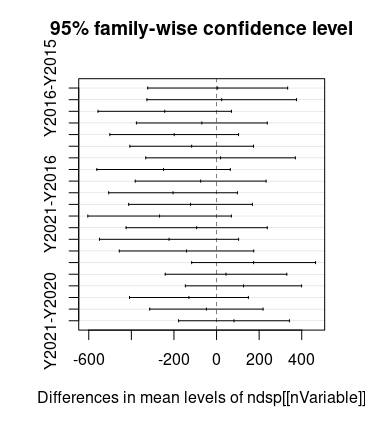
\includegraphics[width=\textwidth, height=\textwidth]{Rplot.png}
    \caption{Distribución de los diferentes niveles del factor \emph{map}}
    \label{fig:yearmap}
  \end{subfigure}
  \hfill
  \begin{subfigure}[b]{0.49\textwidth}
    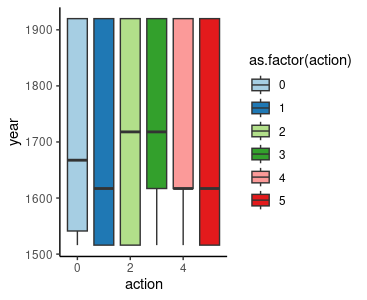
\includegraphics[width=\textwidth, height=\textwidth]{Rplot01.png}
    \caption{Distribución de los diferentes niveles del factor \emph{action}}
    \label{fig:yearaction}
  \end{subfigure}
  \caption{Distribuciones para diferentes niveles de los factores}
\end{figure}

Por último, también podemos ver la distribución de las variables \emph{map} y \emph{action} en función del año (variable \emph{year}) en las Figuras \ref{fig:mapyear} y \ref{fig:actionyear}.

\begin{figure}[!tbp]
  \begin{subfigure}[b]{0.49\textwidth}
    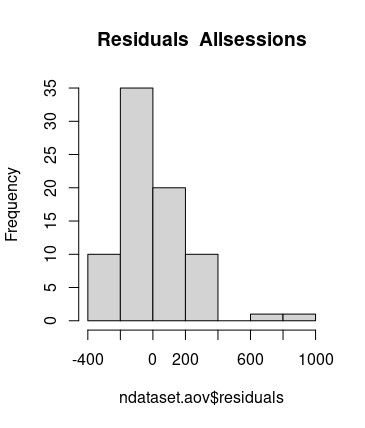
\includegraphics[width=\textwidth, height=\textwidth]{Rplot03.png}
    \caption{Distribución de la variable \emph{map} en función de \emph{year}}
    \label{fig:mapyear}
  \end{subfigure}
  \hfill
  \begin{subfigure}[b]{0.49\textwidth}
    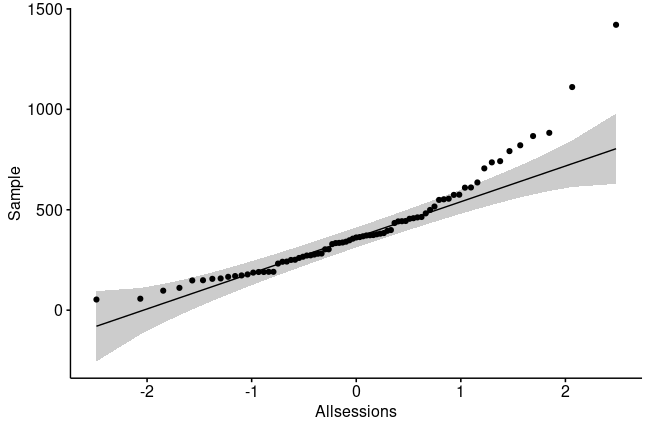
\includegraphics[width=\textwidth, height=\textwidth]{Rplot05.png}
    \caption{Distribución de la variable \emph{action} en función de \emph{year}}
    \label{fig:actionyear}
  \end{subfigure}
  \caption{Distribuciones de las variables \emph{map} y \emph{action} dependiendo del valor de \emph{year}}
\end{figure}

\section{Introducción}

En este estudio inicial se desarrollará un modelo estadístico para determinar el efecto de los parámetros \emph{map} y \emph{action} (dos varibles explicativas) en la variable respuesta \emph{year}.

La relevancia de cada una de las variables en el modelo se determinará por el test \emph{two way ANOVA} con un $5\%$ de nivel de significancia y se empleará la técnica de los \emph{mínimos cuadrados} para estimar los coeficientes del modelo considerado.

\section{Two way ANOVA}

Un resumen de los resultados obtenidos al realizar el test two way ANOVA se muestra en la Tabla \ref{table:3}. Puede observarse que la variable \emph{map} es significante al nivel $0$, que la variable \emph{action} es significante al nivel $0.01$ y que la variable \emph{map:action} (el término de interacción) no es significante. Así pues, puede concluirse que el dataset es homógeneo, es decir, las combinaciones \emph{map:action} son estadísticamente iguales en todos los años considerados.

%Resumen two way ANOVA test:
% latex table generated in R 4.2.2 by xtable 1.8-4 package
% Wed Feb  1 15:19:36 2023
\begin{table}[ht]
\centering
\begin{tabular}{lrrrrr}
  \hline
 & Df & Sum Sq & Mean Sq & F value & Pr($>$F) \\ 
  \hline
map         & 1 & 62918413.58 & 62918413.58 & 2689.15 & 0.0000 \\ 
  action      & 1 & 101244.69 & 101244.69 & 4.33 & 0.0375 \\ 
  map:action  & 1 & 8797.03 & 8797.03 & 0.38 & 0.5398 \\ 
  Residuals   & 47824 & 1118946173.13 & 23397.17 &  &  \\ 
   \hline
\end{tabular}
\caption{Resultados del test two way ANOVA}
\label{table:3}
\end{table}

La notación escalar del modelo ajustado al aplicar el test tiene la siguiente estructura:

\begin{equation}
    y = \beta_0 + \beta_1 \cdot x_1 + \beta_2 \cdot x_2 + \beta_3 \cdot x_1 \cdot x_2 + \epsilon
\label{eq1}
\end{equation}

donde $\beta_0$ es el intercepto, $\beta_1$ y $\beta_2$ son los coeficientes de los efectos principales, $\beta_3$ es el coeficiente del término de interacción, $x_1$ y $x_2$ son los parámetros sometidos a investigación (en este caso, $x_1$ representa el parámetro mapa y $x_2$ representa la acción), $y$ representa el año y $\epsilon$ es el \emph{término error}.

La Tabla \ref{table:4} muestra los valores de los coeficientes de la fórmula que se han obtenido tras ajustar el modelo de regresión a los datos.

%Coeficientes del modelo:
% latex table generated in R 4.2.2 by xtable 1.8-4 package
% Wed Feb  1 15:20:53 2023
\begin{table}[ht]
\centering
\begin{tabular}{rr}
  \hline
 & x \\ 
  \hline
(Intercept) & 1655.03 \\ 
  map & 12.31 \\ 
  action & -1.51 \\ 
  map:action & 0.12 \\ 
   \hline
\end{tabular}
\caption{Coeficientes del modelo}
\label{table:4}
\end{table}

La Figura \ref{fig:interaccion} muestra la interacción entre los parámetros mapa y acción. Así pues, puede observarse que todas las líneras de la gráfica siguen más o menos el mismo patrón, lo que evidencia que no hay una gran interacción entre ambos.

\begin{figure}[h]
    \centering
    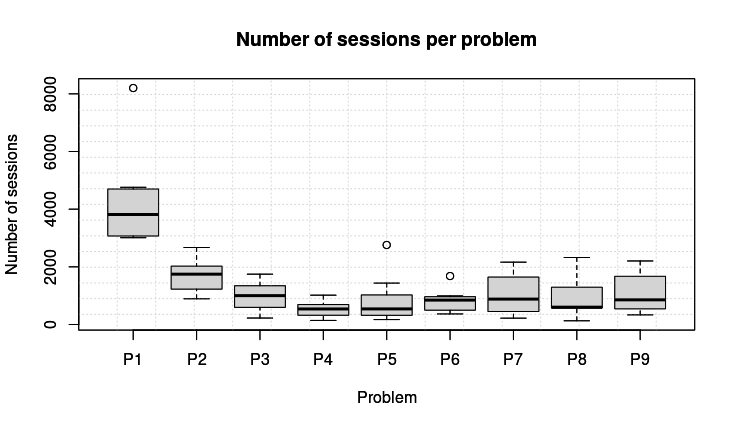
\includegraphics[width=0.60\textwidth]{Rplot06.png}
    \caption{Interacción entre las variables \emph{map} y \emph{action}}
    \label{fig:interaccion}
\end{figure}

% Tukey multiple comparisons of means
% 95% family-wise confidence level
% Fit: aov(formula = year ~ map * action, data = data)
% $map

La Figura \ref{fig:suposiciones} muestra que no se violan las suposiciones que hemos realizado sobre el modelo. La media y la varianza de los residuos no parece que varíe respecto de los valores ajustados. Como consecuencia, conluiré que podemos suponer la homocedasticidad. Además, si nos fijamos en el \emph{Normal Q-Q plot}, puede observarse que los residuos son gaussianos.

\begin{figure}[h]
    \centering
    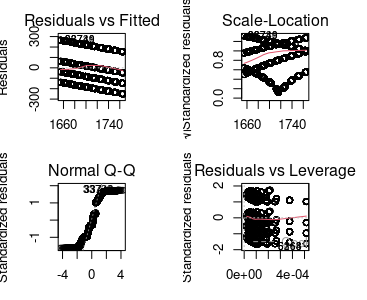
\includegraphics[width=0.60\textwidth]{Rplot07.png}
    \caption{Gráficas diagnósticas del modelo ANOVA}
    \label{fig:suposiciones}
\end{figure}

\end{document}